\documentclass[10pt,a4paper]{article}
\usepackage[english]{babel}
\usepackage[utf8]{inputenc}
\usepackage{fancyhdr}
\usepackage{hyperref}
\usepackage{graphicx}
\usepackage{subcaption}
\usepackage{caption}
\usepackage{cite}
\usepackage{booktabs}
\usepackage{wrapfig}
\usepackage{float}
\usepackage{amsmath}
\usepackage{xcolor}
\usepackage{listings}
\lstset{
	basicstyle=\ttfamily,
	columns=fullflexible,
	frame=single,
	breaklines=true,
	%postbreak=\mbox{\textcolor{red}{$\hookrightarrow$}\space},
}

\restylefloat{table}

\pagestyle{fancy}
\fancyhf{}
\rhead{24-May-2018}
\lhead{Assignment 04}
\rfoot{Page \thepage}

\begin{document}
	\begin{titlepage}
	\centering
	
		{\scshape\LARGE Scientific Experimentation and Evaluation\par}
		\vfill
		{\scshape\Large Assignment: 04\par}
		{\scshape\Large Calibrating an Optical Tracking System\par}
		\vfill
	
		\vfill
		{\Large\itshape Anees Khan (9030423)
			\\Debaraj Barua (9030412)\\
			Md Zahiduzzaman (9030432)
			\par}
		\vfill
	
		{\large 24-May-2018\par}
	\end{titlepage}
	\tableofcontents
	%\listoffigures	
	%\listoftables
	\newpage
	%%%%%%%%%%%%%%%%%%%%%%%%%%%%%%%%%%%%%%%%%%%%%%%%%%%%%%%%%%%%%%%%%%%%%%%
	\section{Relevant Aspects of Experiment}
		\subsection{Setup}
			\subsubsection{Measurement Instruments and Tools}
				\begin{itemize}
					\item We use a standard $10 \times7$ chessboard pattern pasted on a flat board as our calibration grid.
					\item Each grid is of the size 23 mm $\times$ 23 mm.
					\item A Microsoft LiteCam is used to capture the images for calibration.
					\item Camera is mounted on a surface to make sure that it remains stable during operation. 
					\item Camera is connected with the laptop through a USB cable. 
						\item Calibration is done by the camera calibration toolbox for Matlab\cite{calTechCalib}. 
				\end{itemize}
				\begin{figure}[H]
					\begin{subfigure}{0.5\textwidth}
						\centering
						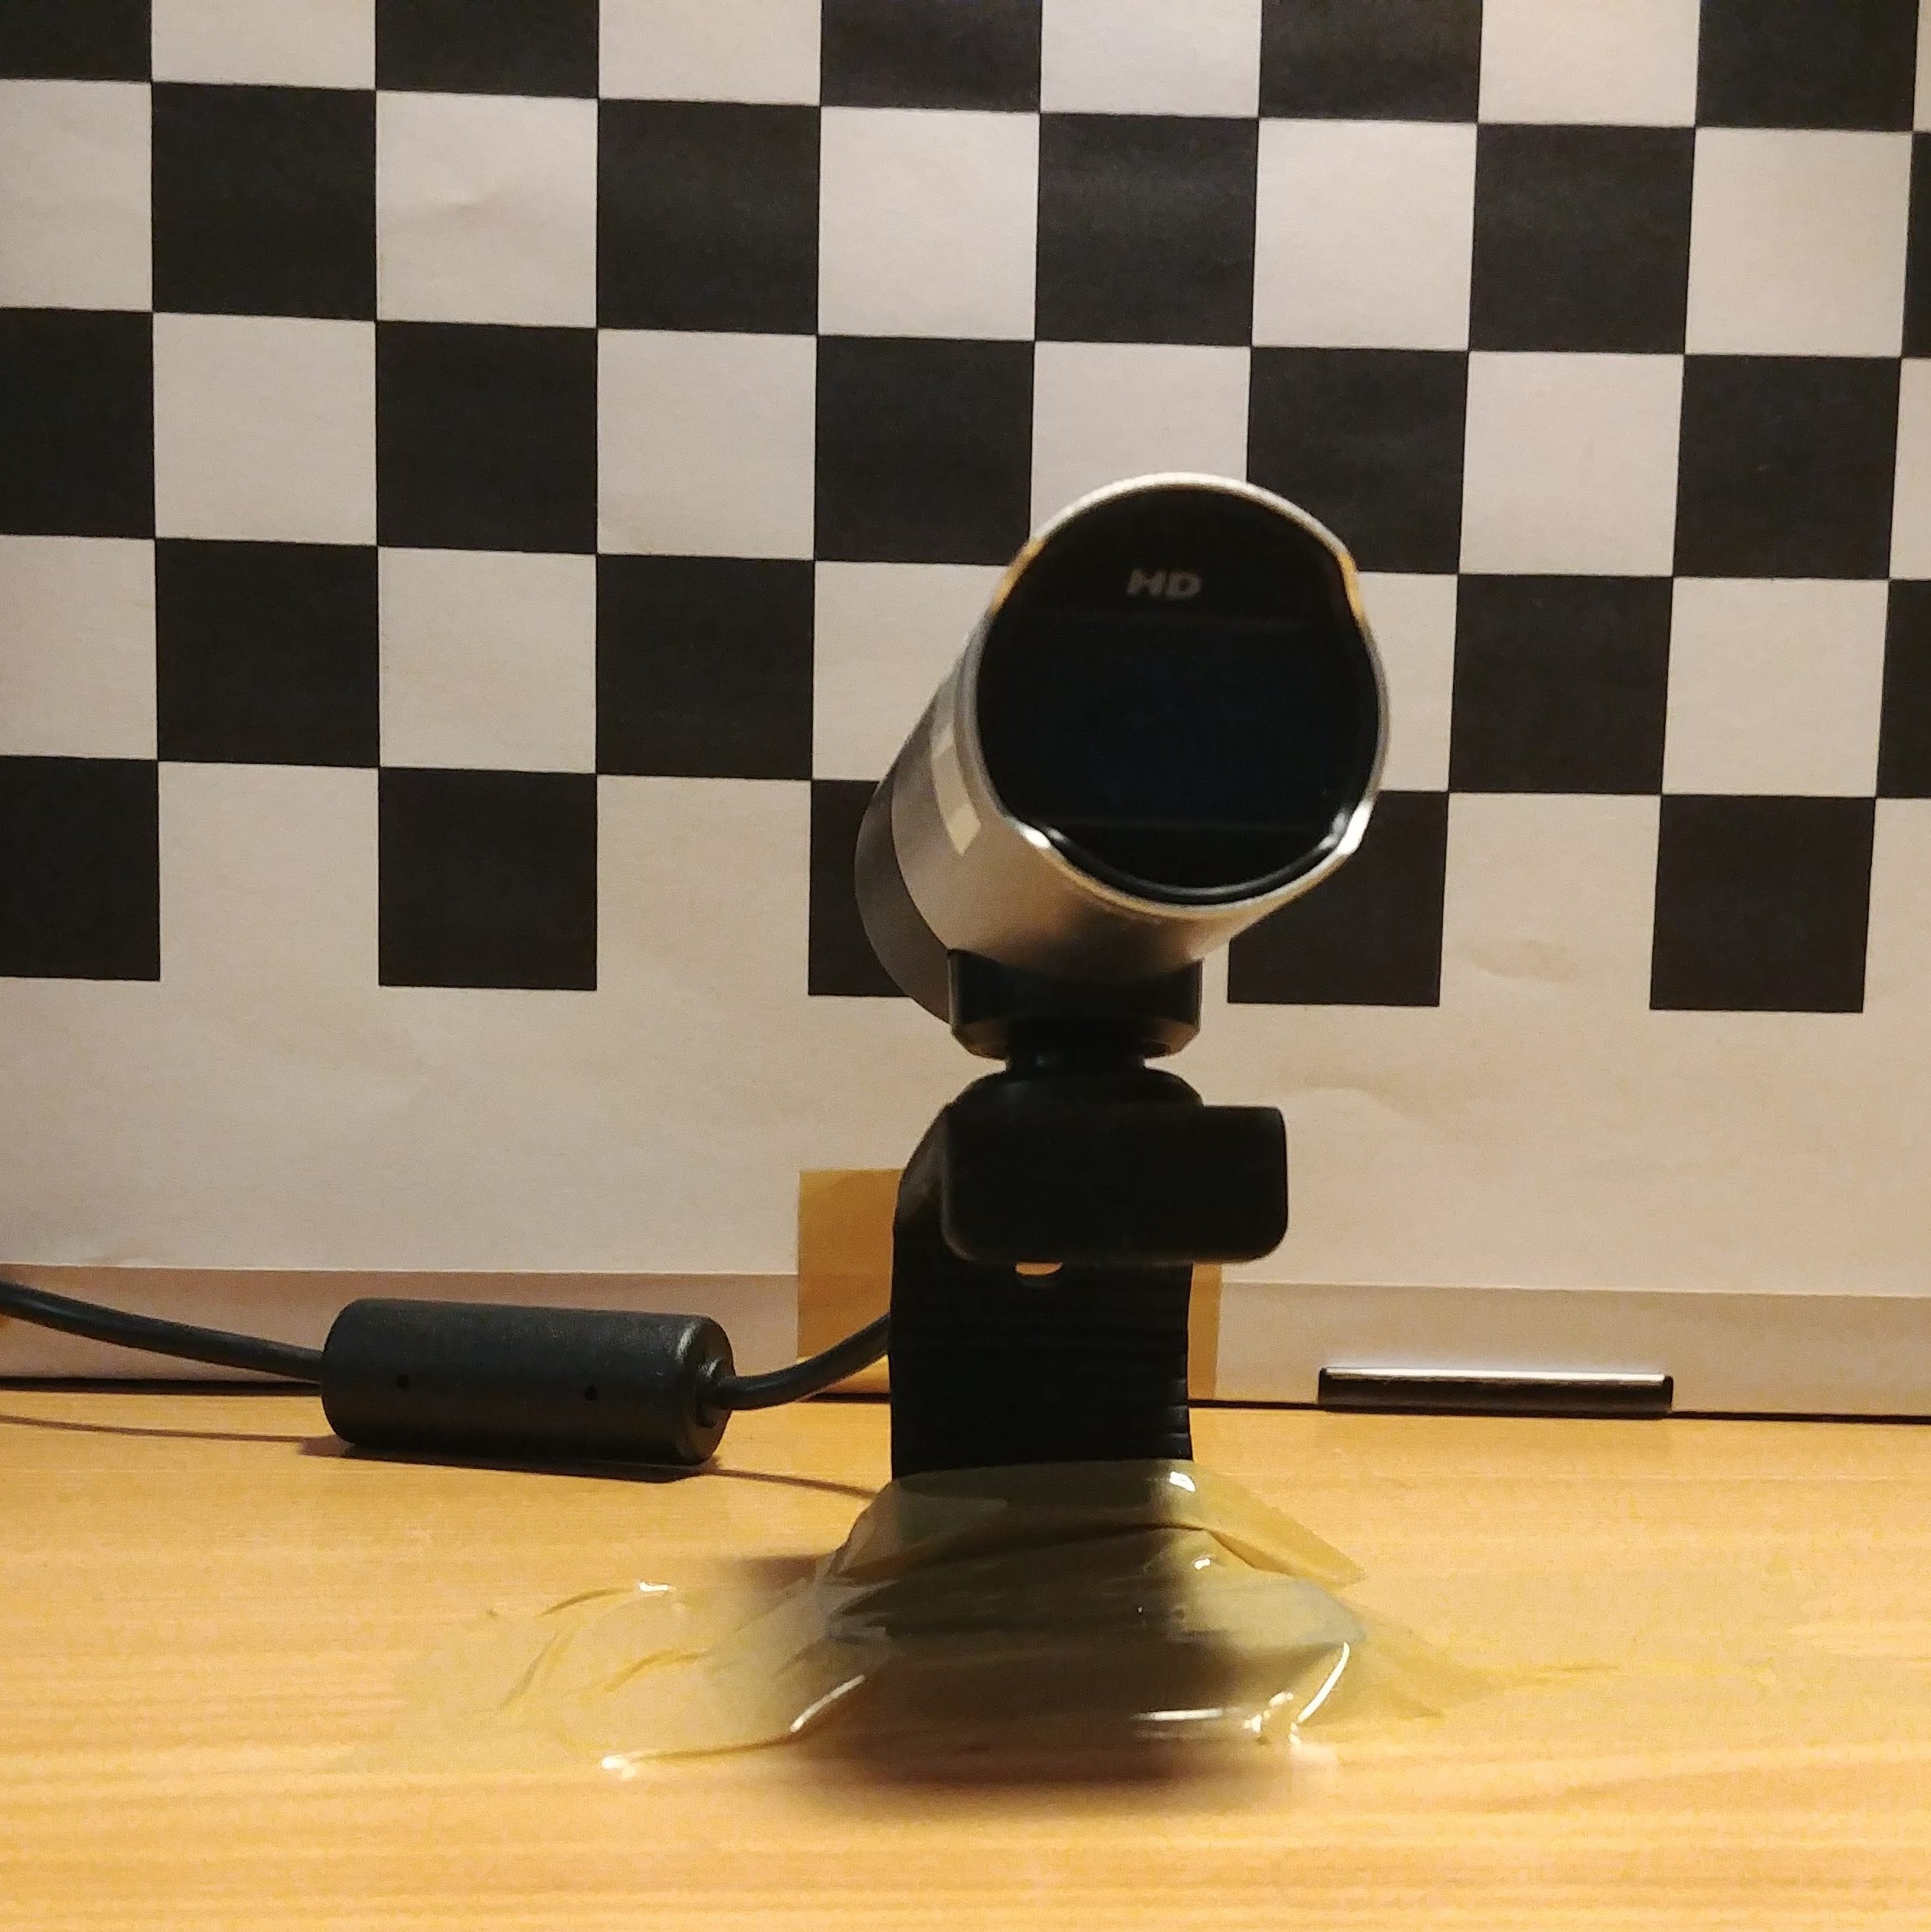
\includegraphics[width=0.8\linewidth]{images/front_cam.jpg}
						\caption{Front View}
						\label{fig:fview}
					\end{subfigure}%
					\begin{subfigure}{0.5\textwidth}
						\centering
						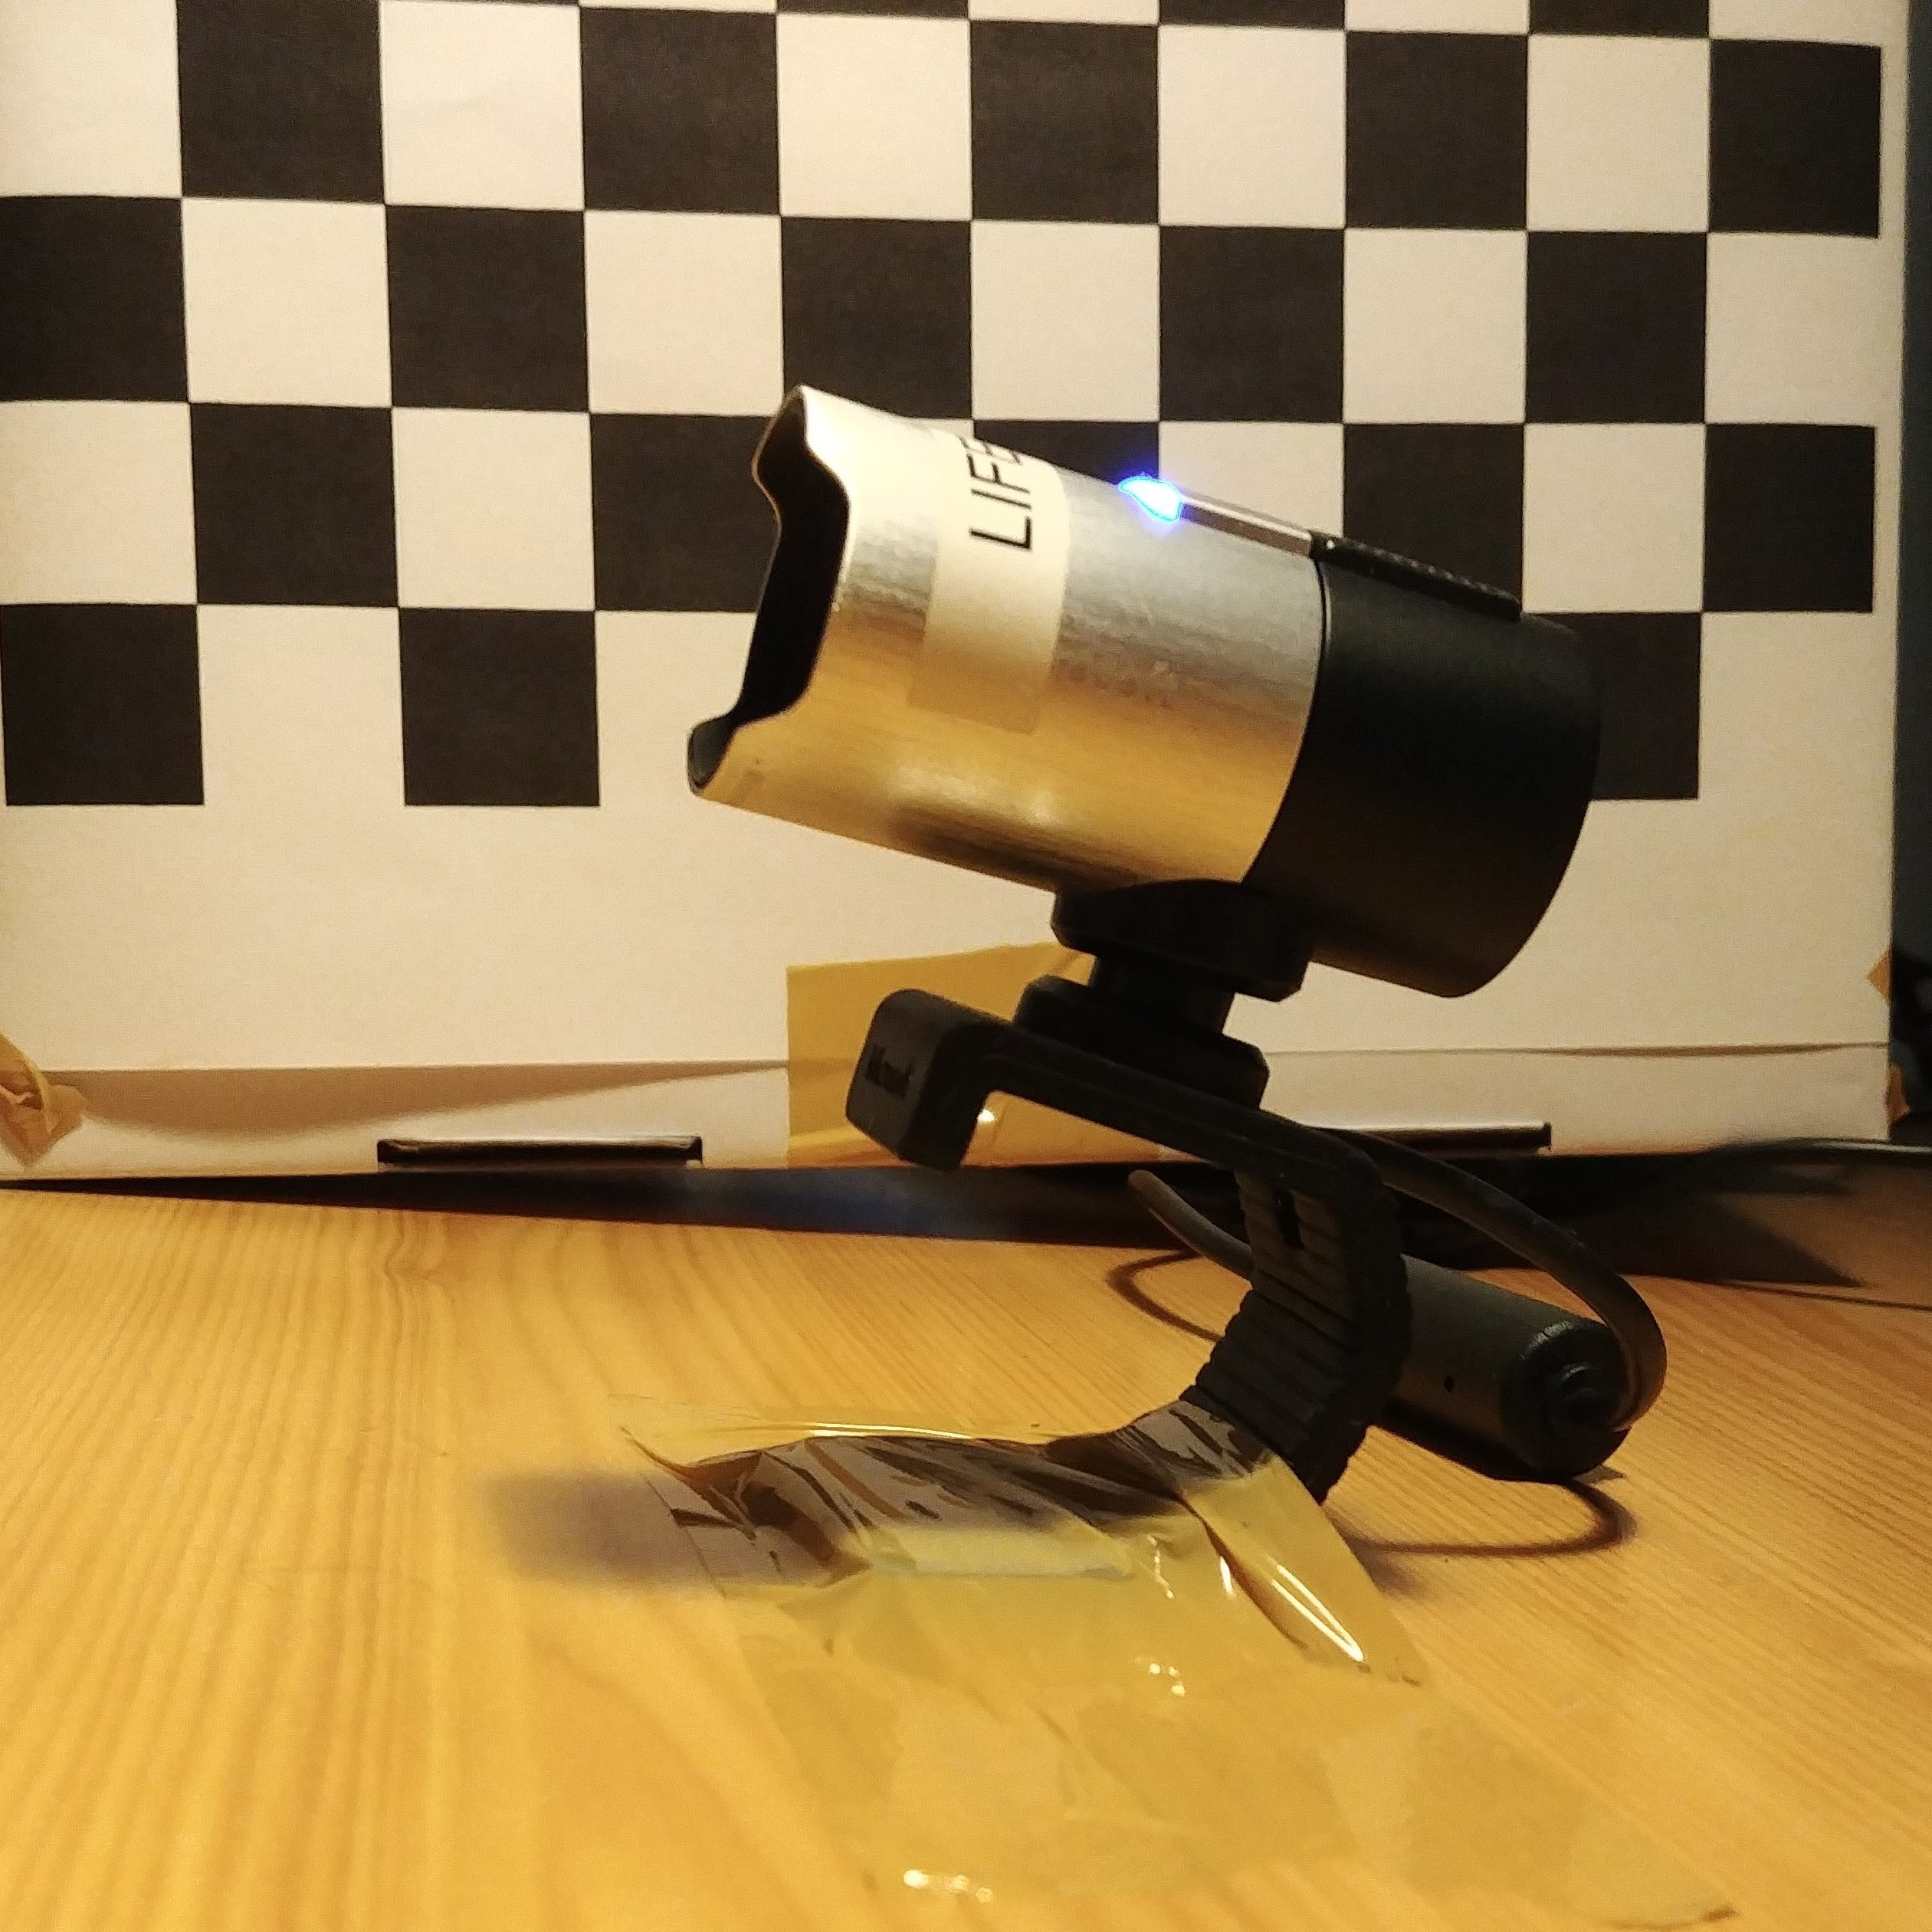
\includegraphics[width=0.8\linewidth]{images/right_cam.jpg}
						\caption{Right View}
						\label{fig:rview}
					\end{subfigure}
					\begin{subfigure}{0.5\textwidth}
						\centering
						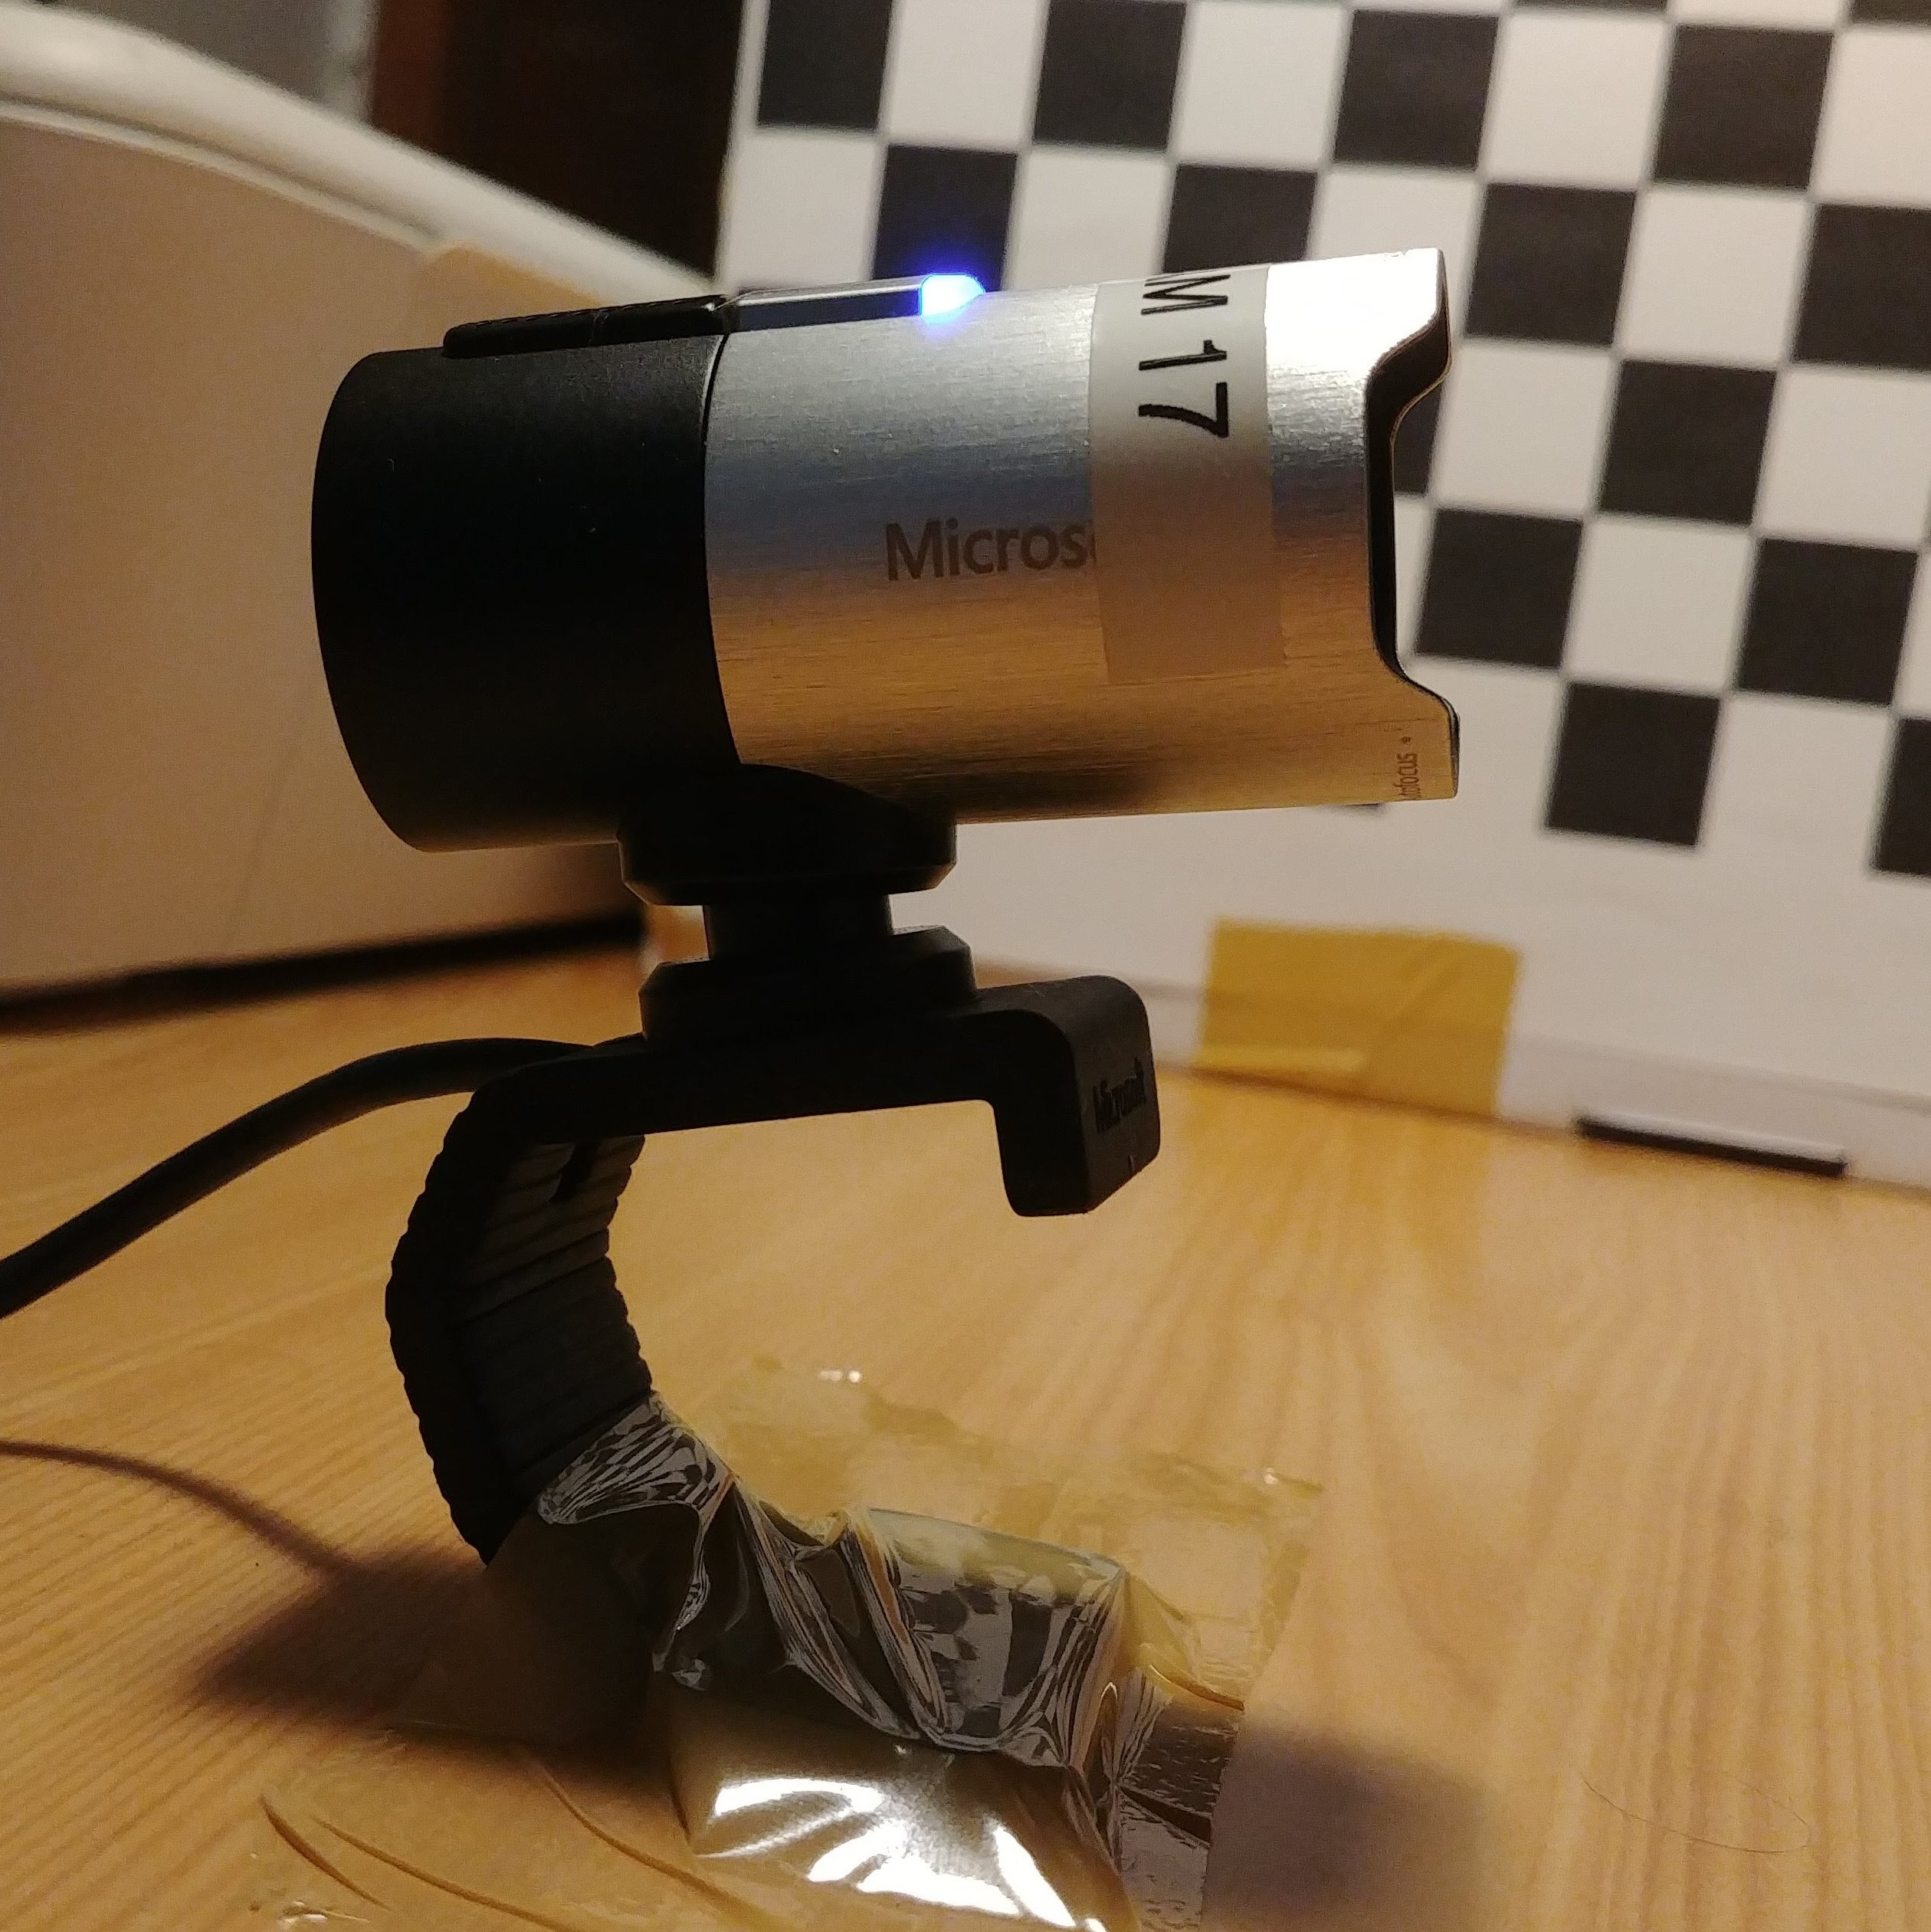
\includegraphics[width=0.8\linewidth]{images/left_cam.jpg}
						\caption{Left View}
						\label{fig:lview}
					\end{subfigure}
					\begin{subfigure}{0.5\textwidth}
						\centering
						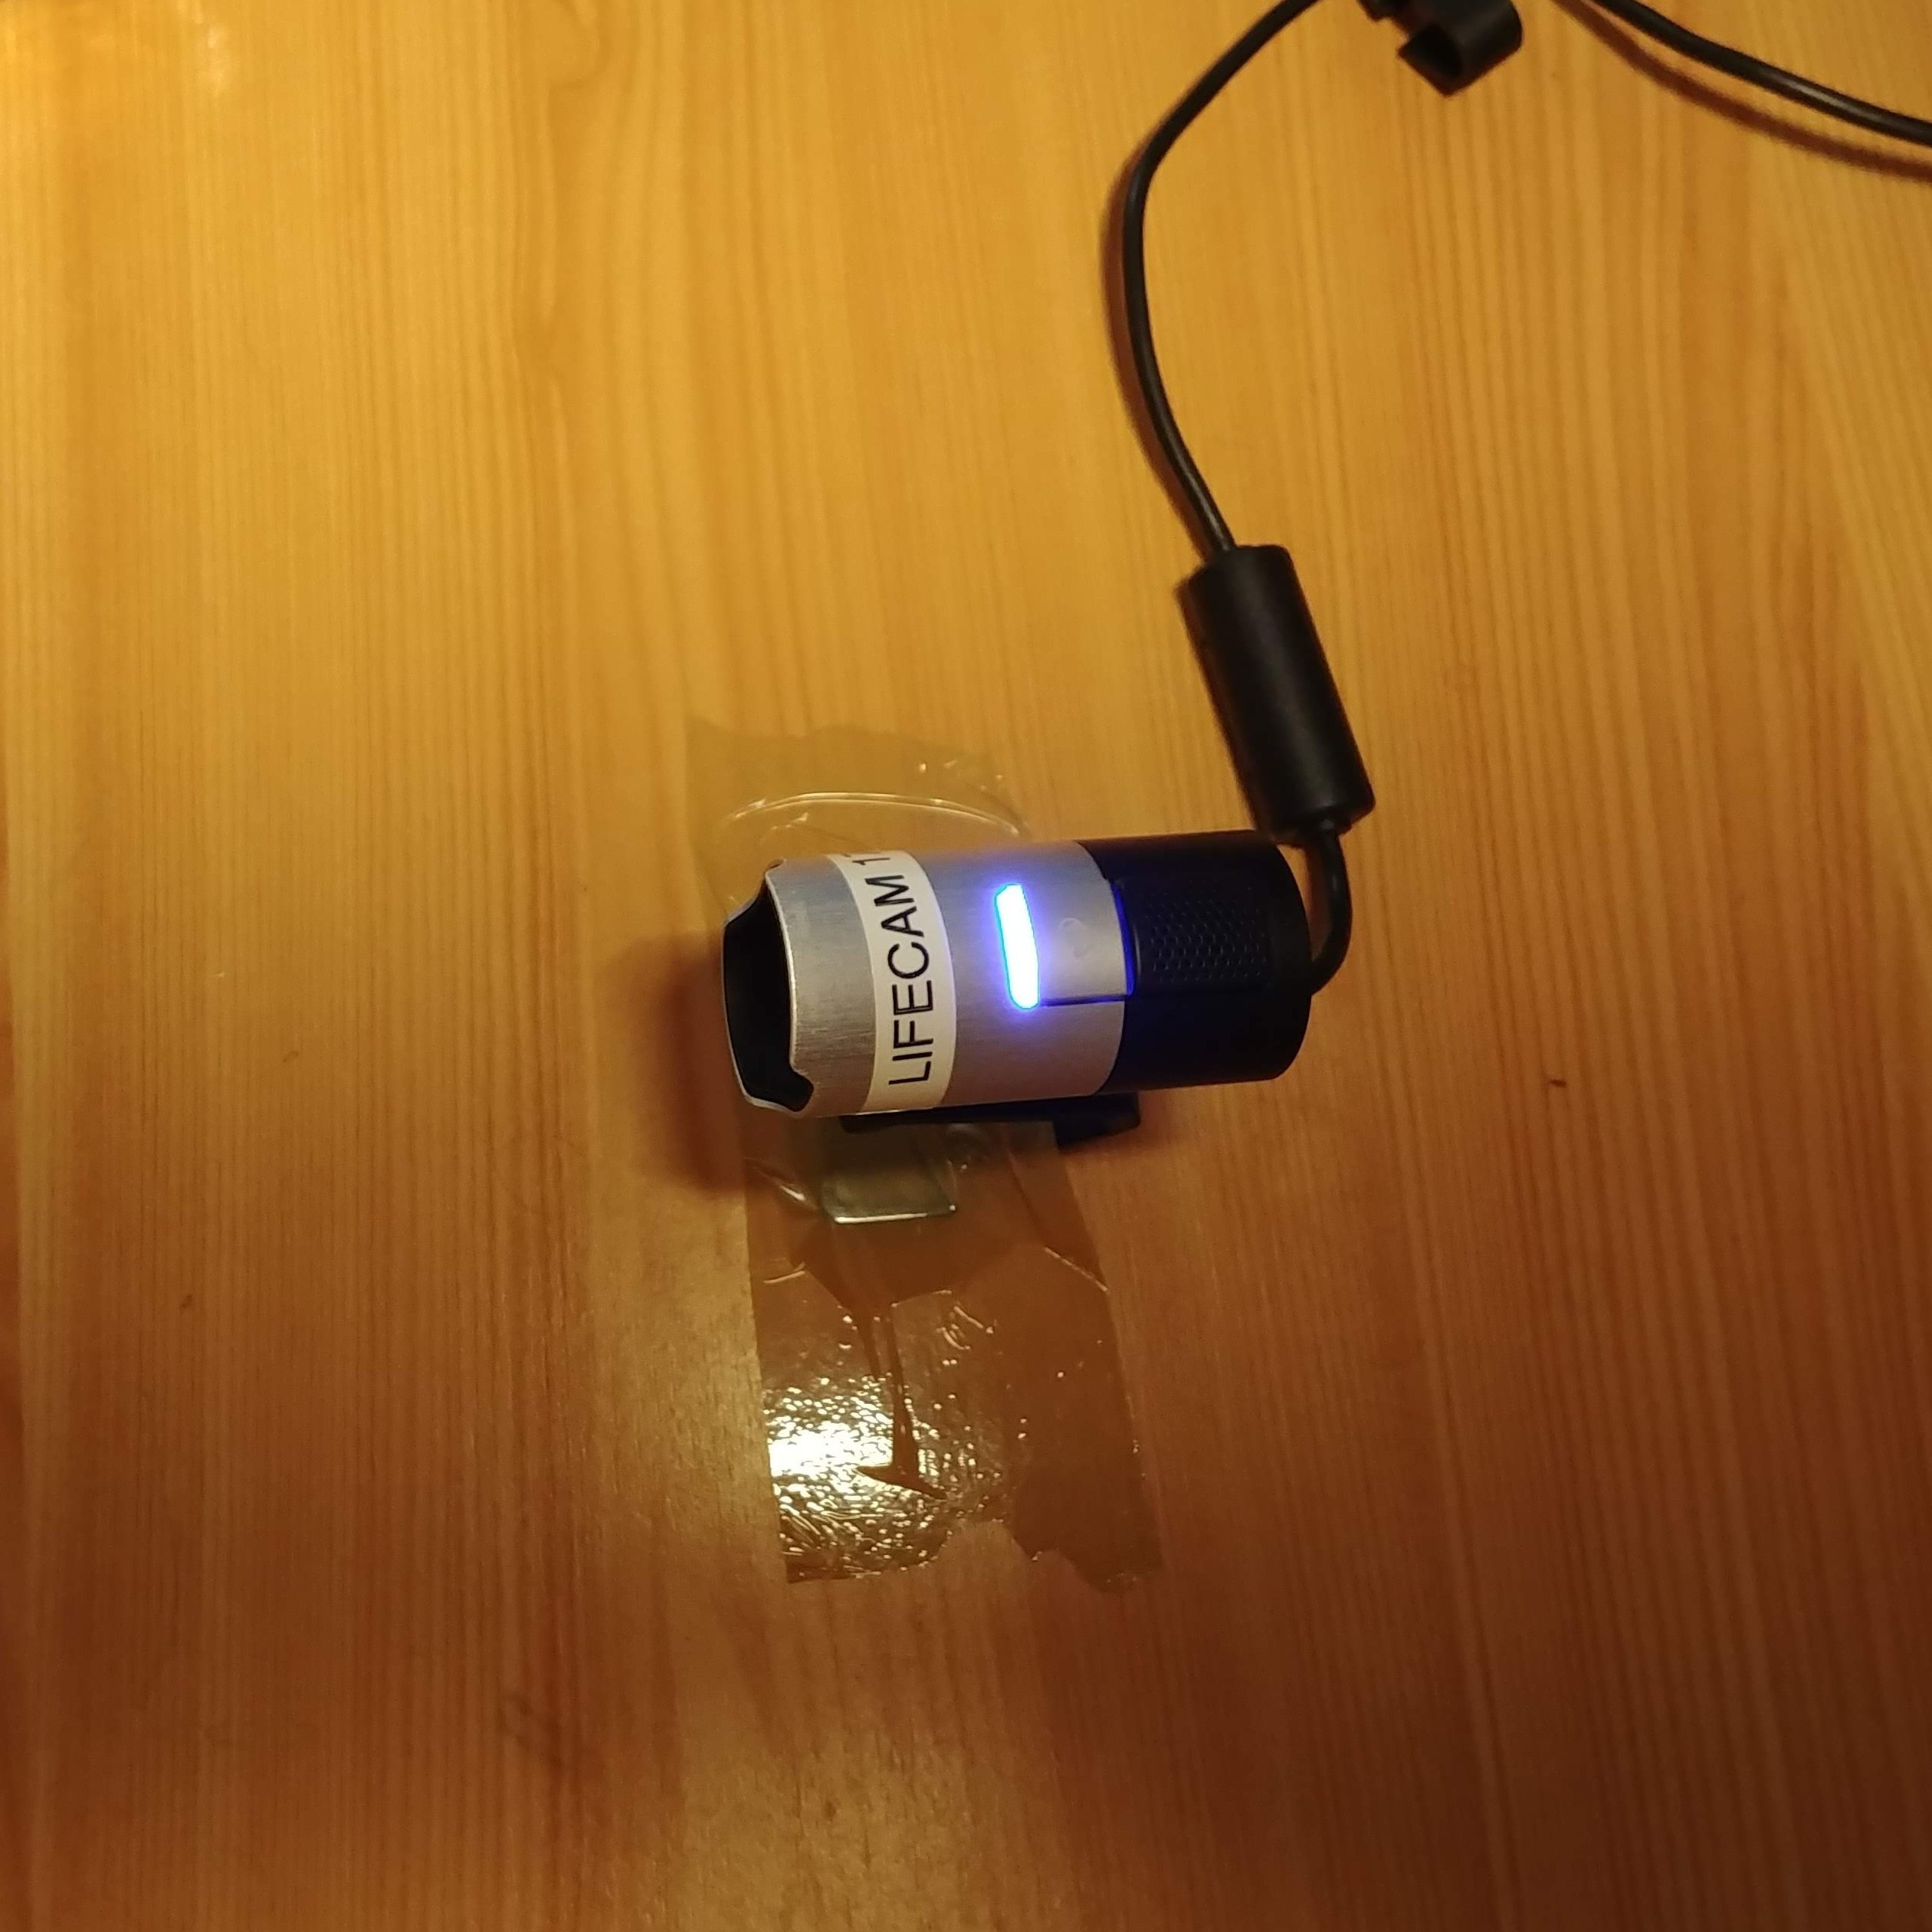
\includegraphics[width=0.8\linewidth]{images/top_cam.jpg}
						\caption{Top View}
						\label{fig:tview}
					\end{subfigure}
					\caption{Camera Setup}
					\label{fig:CamSetup}
				\end{figure}
			\subsubsection{Image Description}
				\begin{itemize}
					\item Images are taken such that the grid appears at different positions and orientation in the field of view of the camera.
					\item The process is repeated multiple times to capture 26 images.
				\end{itemize}			
		\subsection{Description of Parameters}
			\begin{itemize}
				\item The details of the parameters have been given in the documentation of the toolbox. \cite{paramDetails}
				\item \textbf{Intrinsic Parameters}:
					\begin{itemize}
						\item \textit{Focal length}: The focal length in pixels is stored in the 2$\times$1 vector $fc$.
						\item \textit{Principal point}: The principal point coordinates are stored in the 2$\times$1 vector $cc$.
						\item \textit{Skew coefficient}: The skew coefficient defining the angle between the x and y pixel axes is stored in the scalar $alpha\_c$.
						\item \textit{Distortions}: The image distortion coefficients (radial and tangential distortions) are stored in the 5$\times$1 vector $kc$.
						\item \textit{Camera Matrix}, $K$, is given by:
						\[
						\begin{bmatrix}
							fc(1) &     alpha\_c \times fc(1) & cc(1)\\
							0     &     fc(2)                 & cc(2)\\   
							0	  &		0					  & 1
						\end{bmatrix} 						
						\]
						this denotes the intrinsic camera parameters.
					\end{itemize}
				\item \textbf{Extrinsic Parameters}: Is a collection of \textit{rotation matrices} and \textit{translation vectors} corresponding to each image.
			\end{itemize}
		\subsection{Possible Problems or error sources that can disturb the calibration process}
			\begin{itemize}
				\item Errors might arise because of blurred image capture.
				\item Image captured might not sufficiently cover the field of view of the camera.
				\item The lighting condition while capturing the images might not be ideal and may result in non-uniform illumination of the chessboard.
				\item While marking the corners manually during the first stage of calibration,inaccuracies might arise. 
			\end{itemize}
		
	%%%%%%%%%%%%%%%%%%%%%%%%%%%%%%%%%%%%%%%%%%%%%%%%%%%%%%%%%%%%%%%%%%%%%%%		
	\section{Observations and Data}
		\subsection{Image Poses Used}
			\begin{figure}[h]
				\centering
				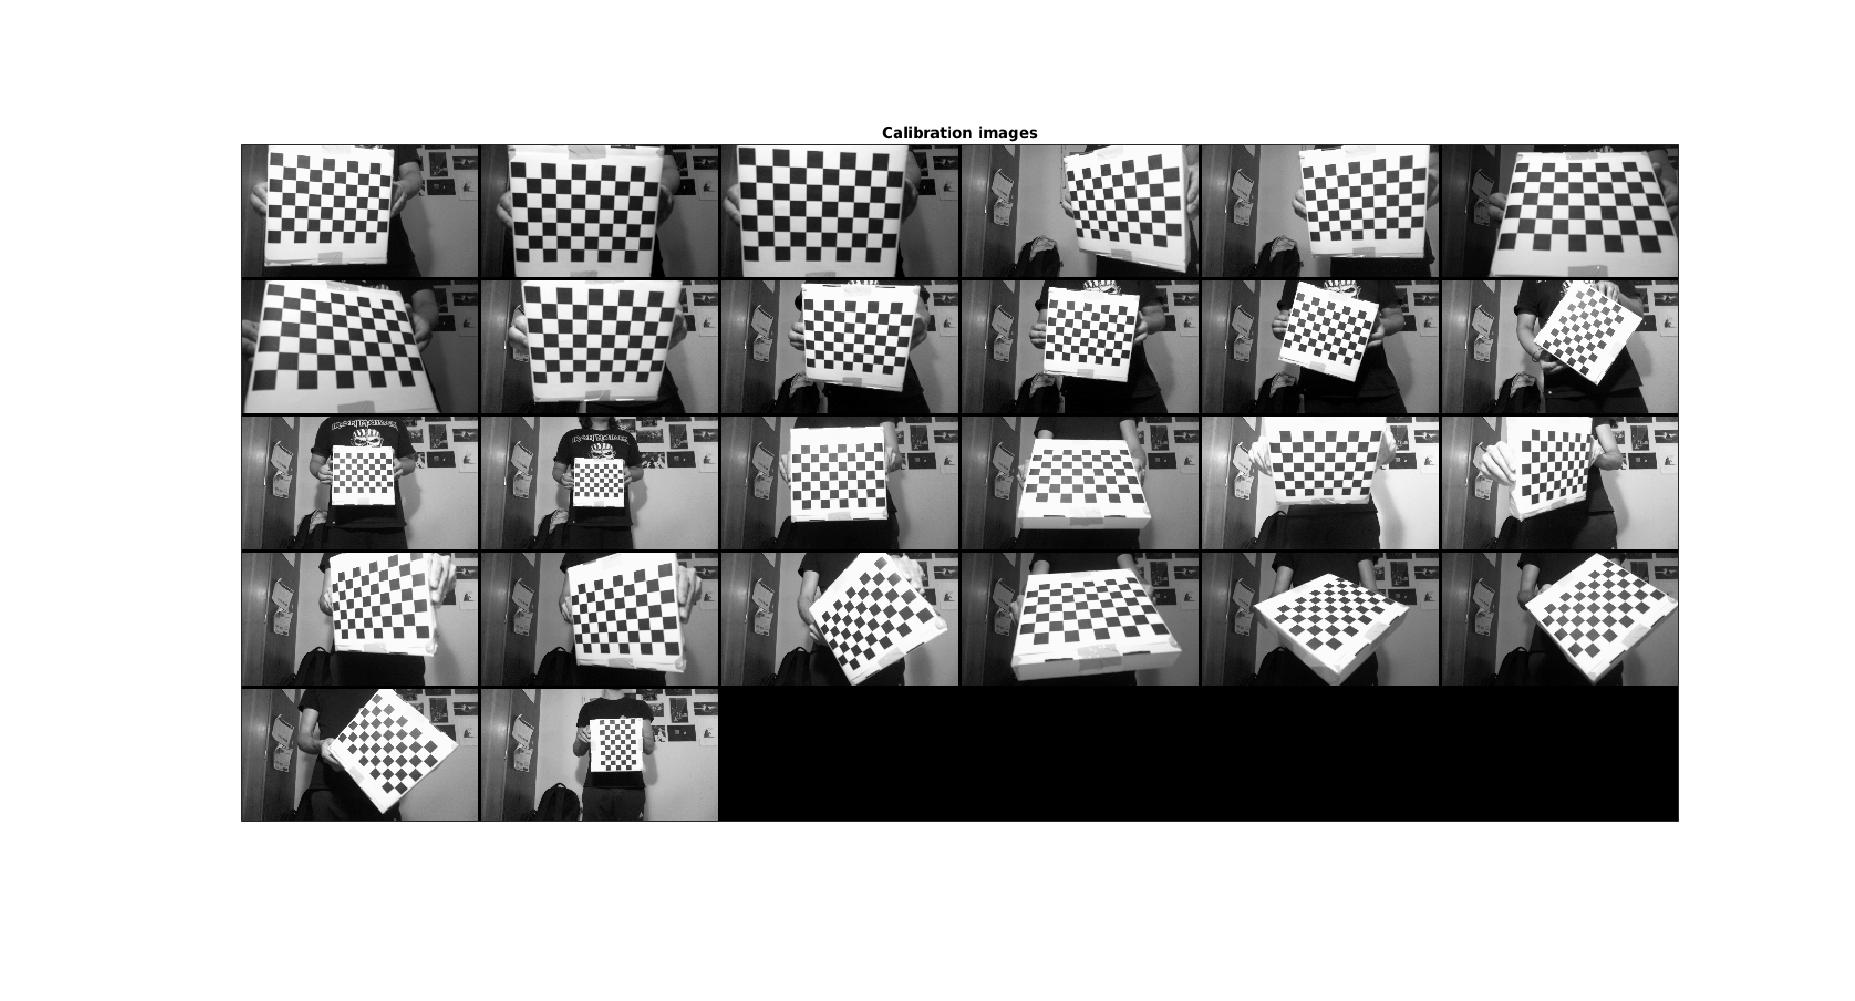
\includegraphics[scale=0.2]{images/calibimages.jpg}
				\caption{Calibration Images}
			\end{figure}
		\subsection{Procedure}
		Following the guidelines described in the toolbox documentation, we went through the below steps:
			\begin{enumerate}
				\item Using all the 26 images we manually identified the corners of each image and ran the calibration script.
				\item Now, we re-project the calibrated corners onto the original images recompute the corners again using different figure size as suggested in the documentation.
				\item On analyzing the re-projection error (image below), we observe many outliers.
					\begin{figure}[h]
						\centering
						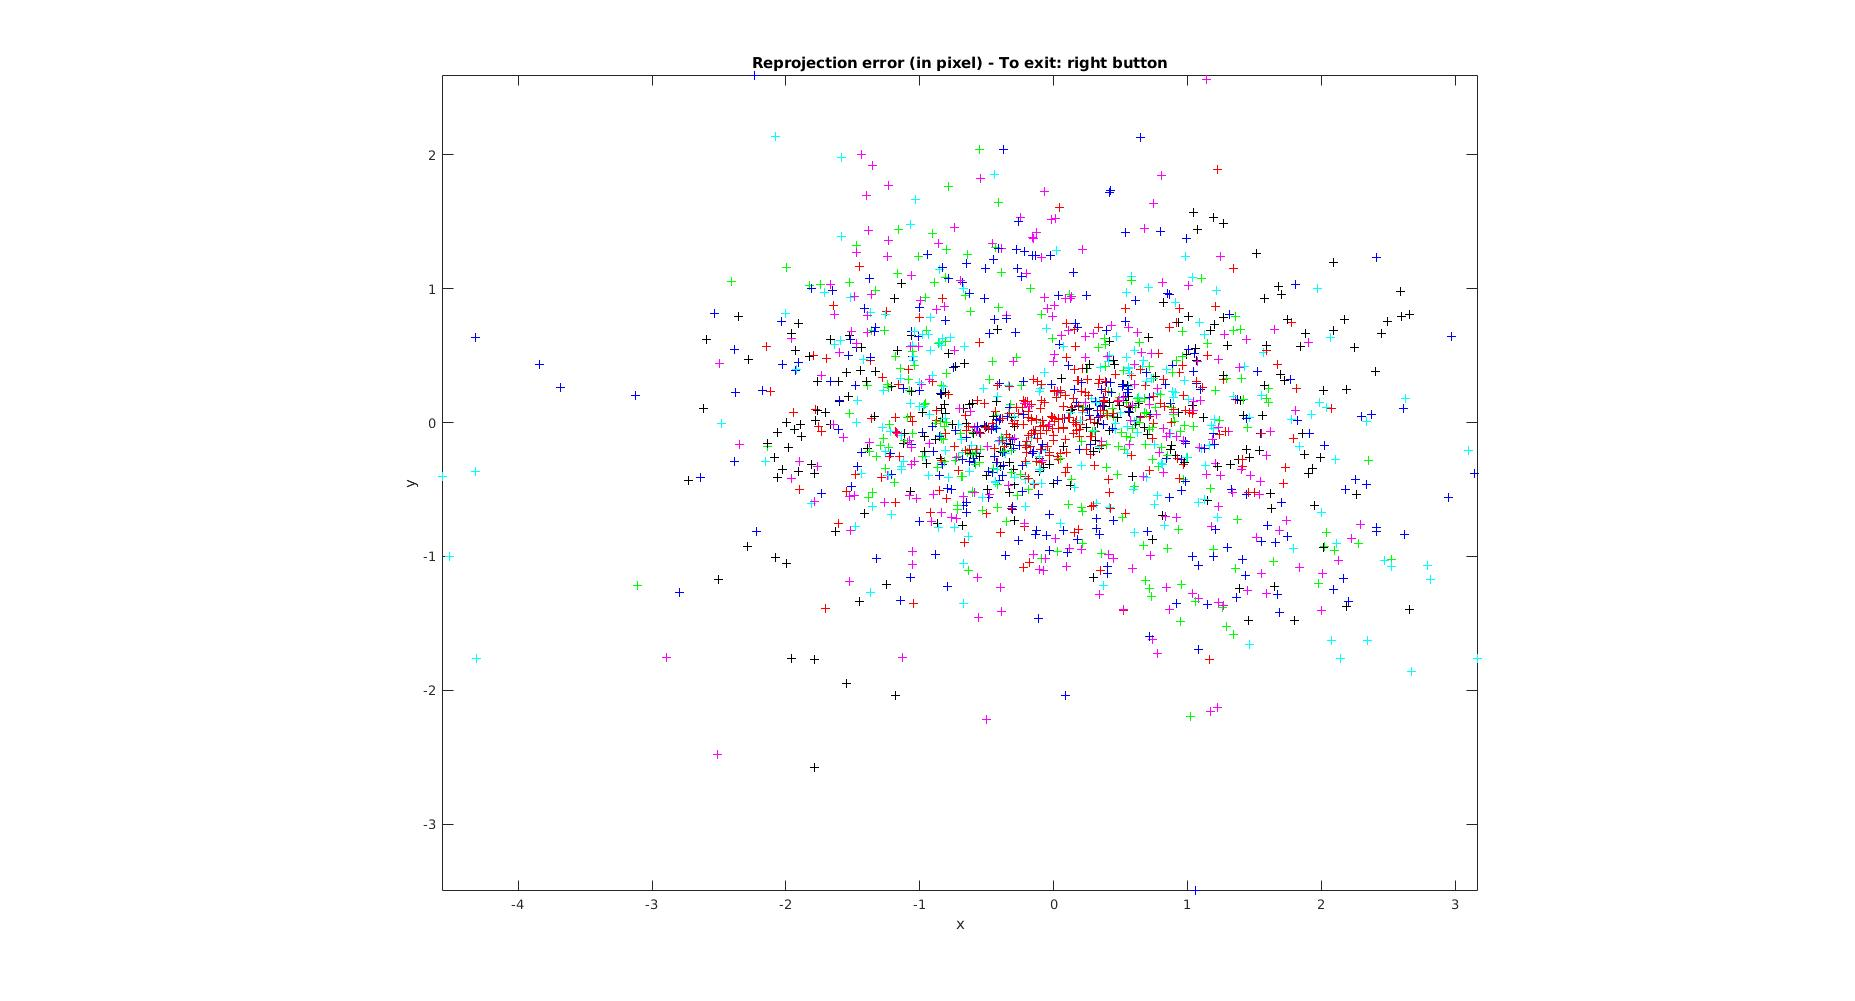
\includegraphics[scale=0.2]{images/analyze_error_initial.jpg}
						\caption{Initial Re-projection Error}
					\end{figure}
				\item After identifying the images corresponding to these outliers we remove 6 images and recompute the corners again and calibrated.
				\item The final re-projection error after this has been found to be significantly improved. The image below has been scaled to similar range as in the previous image.		
					\begin{figure}[h]
						\centering
						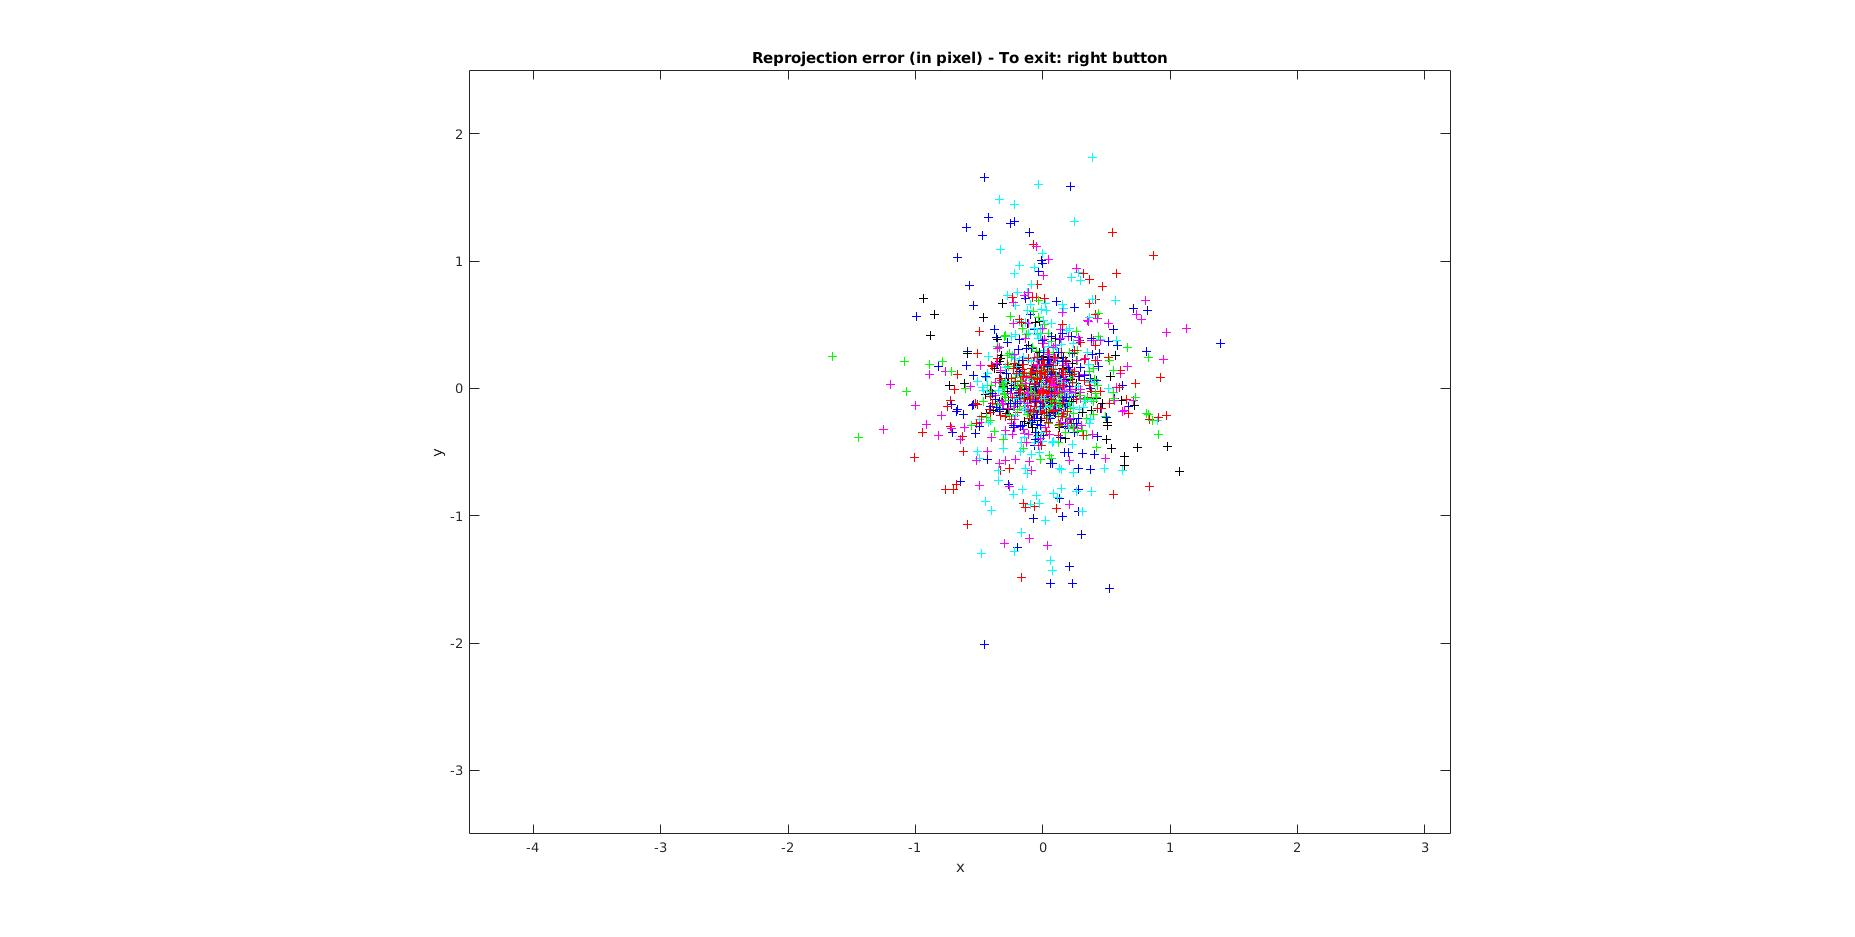
\includegraphics[scale=0.2]{images/analyze_error_final.jpg}
						\caption{Final Re-projection Error}
					\end{figure}		
			\end{enumerate}			
		\subsection{Camera Parameters}
			Calibration results after optimization (with uncertainties):
			\begin{itemize}
				\item Focal Length: $$fc = 
					\begin{bmatrix}975.67762 & 980.32442\end{bmatrix}  +/- 
					\begin{bmatrix}4.01158 &  4.18425 \end{bmatrix} $$
				\item Principal point: $$cc = 
					\begin{bmatrix} 614.92103 &  373.68816\end{bmatrix}  +/- 
					\begin{bmatrix}6.43647 &  4.62420 \end{bmatrix} $$
				\item Skew: $$alpha_c = 
					\begin{bmatrix}  -0.00139 \end{bmatrix}  +/- 
					\begin{bmatrix}0.00079 \end{bmatrix} \implies  \text{angle of pixel axes} = 90.07972 +/- 0.04505 \text{ degrees}$$
				\item Distortion: 
					\begin{align*}
					kc = 
					&\begin{bmatrix}0.01491 &  -0.00391  & 0.00133  & -0.00133 & -0.00000 \end{bmatrix}  +/- \\
					&\begin{bmatrix}0.01137  & 0.03009  & 0.00166  & 0.00231 & 0.00000  \end{bmatrix}
					\end{align*}
				\item Pixel error: $$err = 
					\begin{bmatrix}   0.33413 &  0.41325  \end{bmatrix}
					$$
					The two values are the standard deviation of the re-projection error (in pixel) in both x and y directions respectively.
				\item The extrinsic parameters are included in the 'Calib\_Results.mat' file.
				\item The above parameters were chosen as they provided least pixel error. The procedure to arrive to this has been described in the previous section.
			\end{itemize}	
	\bibliography{references.bib}
	\bibliographystyle{plain}
\end{document}
